\subsection{Cliente} % --------------------- SECTION DEL CLIENTE ---------------------%

 
\subsubsection{Home Page}
Una volta effettuato l'accesso come cliente, verrai reindirizzato alla tua Home Page personale.
Questa Home Page è praticamente identica a quella degli utenti non autenticati, ma con modifiche 
relative alla barra di navigazione in alto. 


\subsection{Barra di navigazione}
La barra di navigazione in alto ti permette di accedere alle sezioni di esplorazione dei ristoranti, 
visualizzare e gestire le proprie prenotazioni, controllare e leggere le notifiche ricevute ed effettuare il ``logout''.

\subsubsection{Esplora}
La sezione ``Esplora'' ti permette di cercare, filtrare e visualizzare tutti i ristoranti registrati su EasyMeal, 
e andare in dettaglio per visualizzare tutte le informazioni relative ad un ristorante. Esattamente come un utente non autenticato.

Una volta entrati nel dettaglio di un ristorante, c'è un'aggiunta speciale: il bottone ``Prenota'' che ti permette di prenotare un tavolo di un ristorante, 
se c'è ancora disponibilità di posti a sedere.

\begin{figure}[htbp]
	\centering
	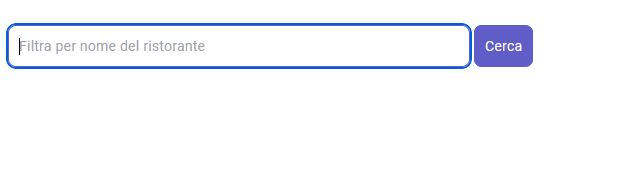
\includegraphics[width=0.5625\textwidth]{./img/Dettaglio.jpg}
	\caption{Bottone di prenotazione di un tavolo di un ristorante}
	% \label{fig:esempio8}
\end{figure}

\subsubsection{Prenotazione di un tavolo}
Una volta cliccato sul tasto prenotazione di un tavolo comparirà un form per inviare la richiesta di prenotazione che sarà accettata o rifiutata dal ristoratore.
Sarà richiesto di inserire il giorno desiderato e un orario compreso tra l'orario di apertura e chiusura del ristorante di quel relativo giorno, inoltre il numero 
di persone che saranno presenti al tavolo.

\begin{figure}[htbp]
	\centering
	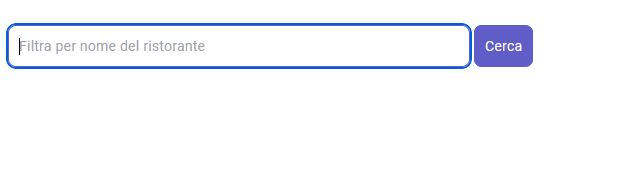
\includegraphics[width=0.5625\textwidth]{./img/Dettaglio.jpg}
	\caption{Form di richiesta di prenotazione di un tavolo di un ristorante}
   %  \label{fig:esempio9}
\end{figure}

\subsubsection{Gestione prenotazioni}
Tornando alla barra di navigazione, cliccando su ``Prenotazioni'' si accede alla pagina di gestione delle prenotazioni.
In cui si ha un elenco di tutte le prenotazioni effettuate, con la possibilità di visualizzare in dettaglio una prenotazione, semplicemente cliccando su di essa.
In questa lista si possono visualizzare le prenotazioni in attesa di conferma, quelle confermate e quelle rifiutate, quindi si possono visualizzare il nome della 
prenotazione, l'orario in cui è stata effettuata, lo stato della prenotazione e il ristorante a cui si riferisce, e lo stato della prenotazione.

\begin{figure}[htbp]
	\centering
	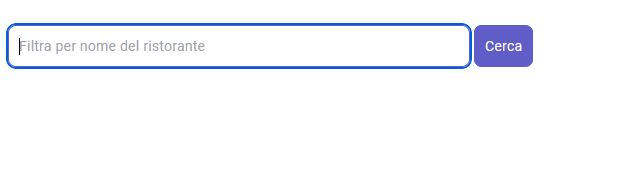
\includegraphics[width=0.5625\textwidth]{./img/Dettaglio.jpg}
	\caption{Visualizzazione delle prenotazioni effettuate}
	% \label{fig:esempio10}
\end{figure}

\subsubsection{Eliminazione prenotazione}
Nel caso in cui si è stati aggiunti ad un prenotazione e non si vuole partecipare o la si vuole cancellare bisognerà semplicemente cliccare sul pulsante ``X'' 
che compare a destra di ciascuna prenotazione nella lista.

\begin{figure}[htbp]
	\centering
	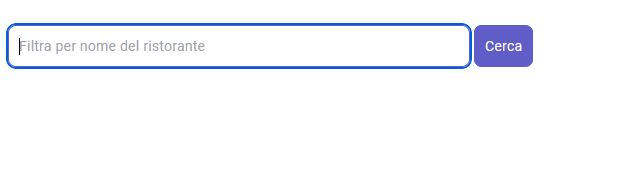
\includegraphics[width=0.5625\textwidth]{./img/Dettaglio.jpg}
	\caption{Pulsante di eliminazione di una prenotazione}
	% \label{fig:esempio11}
\end{figure}

\subsubsection{Accettazione prenotazione}
Nel caso contrario, ovvero nel caso in cui si è stati aggiunti ad una prenotazione e si desidera confermare la presenza bisognerà semplicemente cliccare sul pulsante ``V'', 
che compare a destra di ciascuna prenotazione nella lista.

\begin{figure}[htbp]
	\centering
	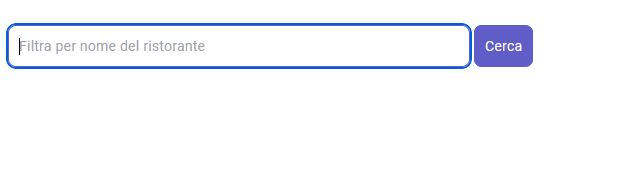
\includegraphics[width=0.5625\textwidth]{./img/Dettaglio.jpg}
	\caption{Pulsante di accettazione di una prenotazione}
	% \label{fig:esempio12}
\end{figure}

\subsubsection{Notifiche}
Tornando alla barra di navigazione, cliccando su ``Notifiche'' si accede alla pagina di visualizzazione delle notifiche.
In cui si ha la possibilità di filtrare le notifiche in base a Nuove o Lette, semplicemente cliccando sopra nuove o lette. Per default 
saranno visualizzate quelle nuove in base all'ordine di ricezione. 
Per eliminare la spunta di novità su una notifica basterà cliccare su di essa.

\begin{figure}[htbp]
	\centering
	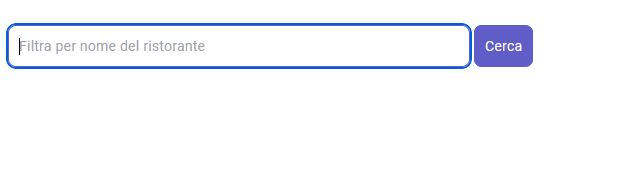
\includegraphics[width=0.5625\textwidth]{./img/Dettaglio.jpg}
	\caption{Visualizzazione delle notifiche ricevute}
	% \label{fig:esempio13}
\end{figure}

\subsubsection{Logout}
L'ultima funzionalità presente nella barra di navigazione di un cliente è la possibilità di effettuare il ``logout'' cliccando sul pulsante ``Logout''.
Una volta effettuato con successo si sarà reindirizzati nella Home Page di un classico utente non autenticato con le relative funzionalità.
